\documentclass[10pt,a4paper,titlepage]{article}
\usepackage[utf8]{inputenc}
\usepackage{amsmath}
\usepackage{amsfonts}
\usepackage{amssymb}
\usepackage{makeidx}
\usepackage{enumitem}
\usepackage{graphicx}
\usepackage{longtable}
\usepackage[hidelinks]{hyperref}

%this is a command used in the title template
\newcommand{\HRule}{\rule{\linewidth}{0.5mm}}

%questo fa in modo che le liste numerate (tipo goals o functional requirements) siano allineate come le altre
\setenumerate{leftmargin=*, labelindent=\parindent}

%questo genera il toc, ricorda di eseguire due volte
\makeindex

\begin{document}
\begin{titlepage}
\begin{center}

%logo

\includegraphics[width=0.30\textwidth]{./images/logo}~\\[1cm]
\textsc{\LARGE Politecnico di Milano}\\[1.5cm]

\textsc{\Large Software Engineering 2 Project}\\[0.5cm]

% Title
\HRule \\[0.4cm]
{ \Huge \bfseries MeteoCal \\[0.4cm] }
{ \huge \bfseries Design Document \\[0.4cm] }
\HRule \\[1.5cm]

% Author
\begin{flushright}
\noindent
\large
\emph{Authors:}\\
Andrea \textsc{Celli}\\
Stefano \textsc{Cereda}
\end{flushright}
\vfill

% Bottom of the page
{\large \today}

\end{center}
\end{titlepage}

\part{Introduction}

\section{Purpose}
This document introduces the general functionalities of MeteoCal. This project is developed for the Software Engineering 2 course held at Politecnico di Milano. The intended audience is composed by people who want to organize their activities in a calendar and manage them according to the weather forecast. Individuals that will participate actively in the project are Software Engineering students for the moment, and in the future anyone wishing to use such a system.
The main functionalities of MeteoCal will be:
\begin{itemize}
\item An on-line calendar.
\item A system to manage activities according to weather forecast.
\end{itemize}

\section{Scope}
The software product that will be delivered is MeteoCal, a web application intended to be used by people to schedule their appointments and rearrange them based on weather forecasts.
The main objectives of MeteoCal are:
\begin{itemize}
\item Allow a user to manage (create, delete or update) his events.
\item Allow a user to invite other users to his events and allow the invited users to either accept or decline the invitation.
\item In case of bad weather the system has to notify all the event's participants one day in advance
\item Allow a user to define his calendar as public or private, if the calendar is public the other users will be able to see when the user is busy.
\item Allow a user to define his events as public or private, if an event is public other users will be able to see its details.
\item Three days before the event in case of bad weather the system will propose to the event creator the closest sunny day.
\end{itemize}
MeteoCal will provide general functionalities for managing:
\begin{itemize}
\item Users: MeteoCal will manage personal data of the users. MeteoCal will manage registering, logging in/out and the modification of personal data.
\item Calendar: MeteoCal will manage a calendar for each user. User will be able to create, update and delete an event and to see other people's events. MeteoCal will also manage event invitation.
\item Weather: MeteoCal will manage weather forecasts and send notifications to event's participants one day in advance in case of bad weather. It will also have to propose an alternative schedule to the event creator with three day of advance.
\end{itemize}
MeteoCal will have the following limitations (probably developed in future versions):
\begin{itemize}
\item Synchronization with other calendars: MeteoCal will not support the import/export of user's calendar.
\item Multiple calendars: a user will have exactly one calendar.
\item In case of bad weather, MeteoCal will ask if the proposed schedule is fine only to the event creator, and not to all the event participants.
\item Avoid events conflicts: MeteoCal will not check if a new event overlaps with an existing one.
\item Periodical weather updates: MeteoCal will not send a periodical update of the weather forecast.
\end{itemize}
MeteoCal will have the following goals:
\begin{enumerate}[label = G\arabic*:]
\item Allow the registration of new users
\item Allow users to view, create, update and delete events in their calendar
\item Allow users to invite other users to their events
\item Allow invited users to either accept or decline the invitation
\item Allow users to see other users public calendar
\item Allow users to see other users public events details
\item Send a notification to all the participants one day in advance in case of bad weather
\item Propose an alternative schedule to the event creator three day in advance in case of bad weather
\item Notify all the event's participant in case the creator changes some details
\item Allow users to modify their data
\end{enumerate}
\section{Definitions and acronyms}

\subsection{Definitions}
\begin{itemize}
\item Calendar: a calendar is the agenda of an user
\item Event: a task that a user has into his calendar
\item Registered user: a user that has created an account on MeteoCal
\item Logged user: a registered user that has performed the login process
\item Unlogged user: either a non registered user or a registered user that is logged out of the system
\end{itemize}

\subsection{Acronyms and abbreviations}
\begin{itemize}
\item MeteoCal: Meteorological Calendar
\item G: Goal
\item JVM: Java Virtual Machine
\item JEE: Java Enterprise edition
\item DBMS: Database management system
\item AS: Application server
\item FR: Functional requirement
\item NFR: Non-functional requirement
\end{itemize}

\section{Reference documents}
\begin{itemize}
\item Alloy model file: MeteoCal.als
\end{itemize}

\section{Overview}
This document is organized as follows:
\begin{itemize}
\item Part 1, Introduction: provides a synopsis of the software product to be developed.
\item Part 2, Overall Description: describes the general factors that affect the software product and its requirements.
\item Part 3, Specific Requirements: contains the artifacts generated by the analysis. It describes all of the software requirements to a level of detail sufficient to be externally perceivable.
\item Part 4, Appendixes: provides supporting information about how the alloy model contributed to the requirement analysis and analysis model.
\end{itemize}

\clearpage
\part{Overall Description}
This section does not describe specific requirements, but puts the product into perspective and provides a background for specifying concrete requirements in the next section of this document.

\section{Product Perspective}
The software product is a complete self-contained system and it is not part of any other larger system. However in the future it may offer external interfaces to other calendars.

\subsection{System Interfaces}
The software product does not provide any external interface.

\subsection{User interfaces}
The software product will present the following page layouts as the user interface. These
page layouts offer a minimalistic approach to design and navigation.
This is the MeteoCal homepage:

\vspace{2mm}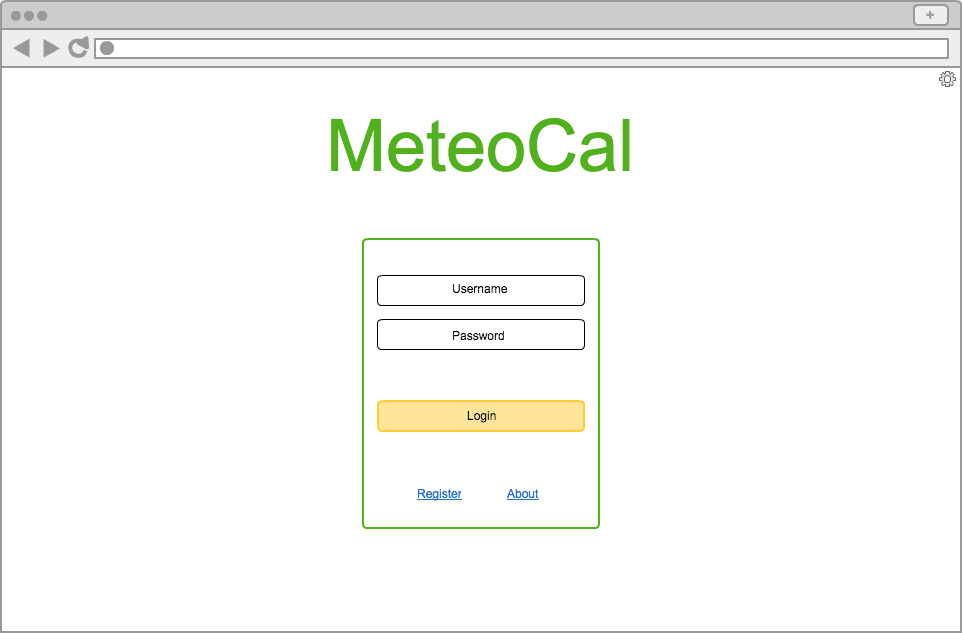
\includegraphics[width={\linewidth}]{./UI_mockups/01-login.png}\vspace{3mm}

Here the users can log into the system giving his data. The user can also navigate to the “about” page:

\vspace{3mm}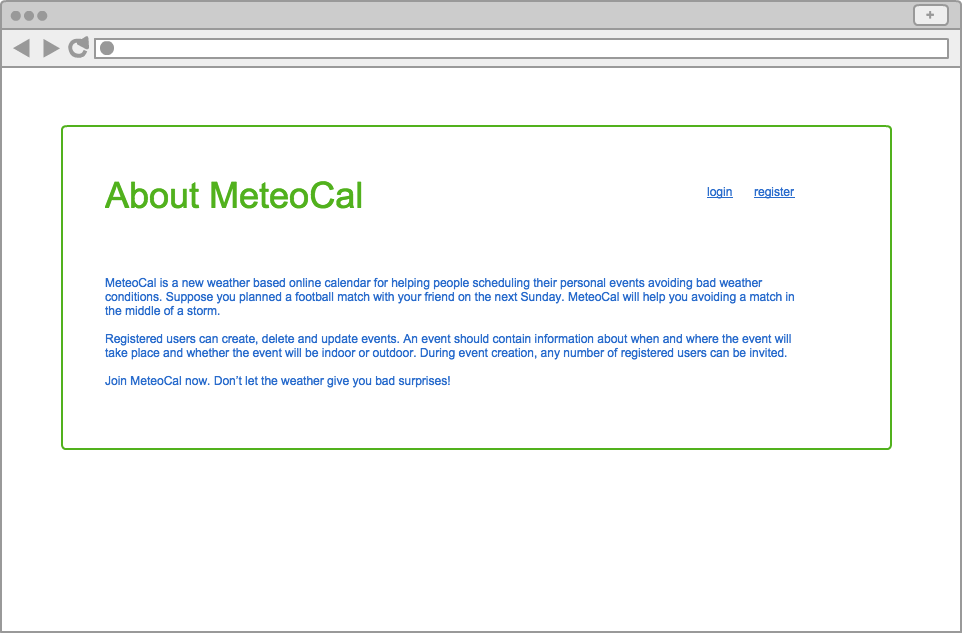
\includegraphics[width={\linewidth}]{./UI_mockups/02-about.png}\vspace{3mm}

Where a brief description of the MeteoCal service is provided.
From both the “homepage” and the “about” pages the user can navigate to “register” page:

\vspace{3mm}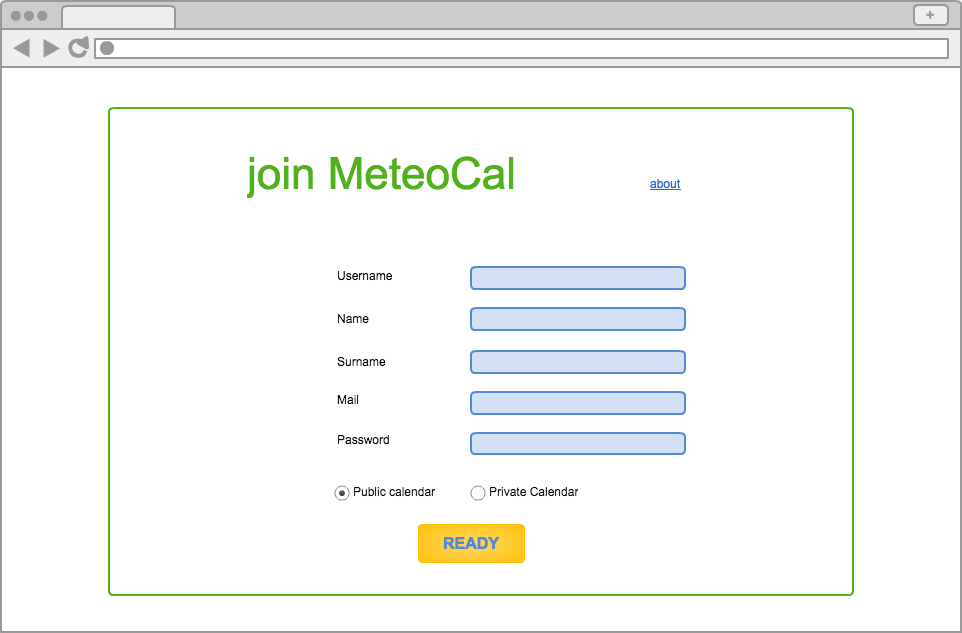
\includegraphics[width={\linewidth}]{./UI_mockups/03-register.png}\vspace{3mm}

Where new users can register to the system by submitting their data.
Once logged the users see the “logged user homepage”:

\vspace{3mm}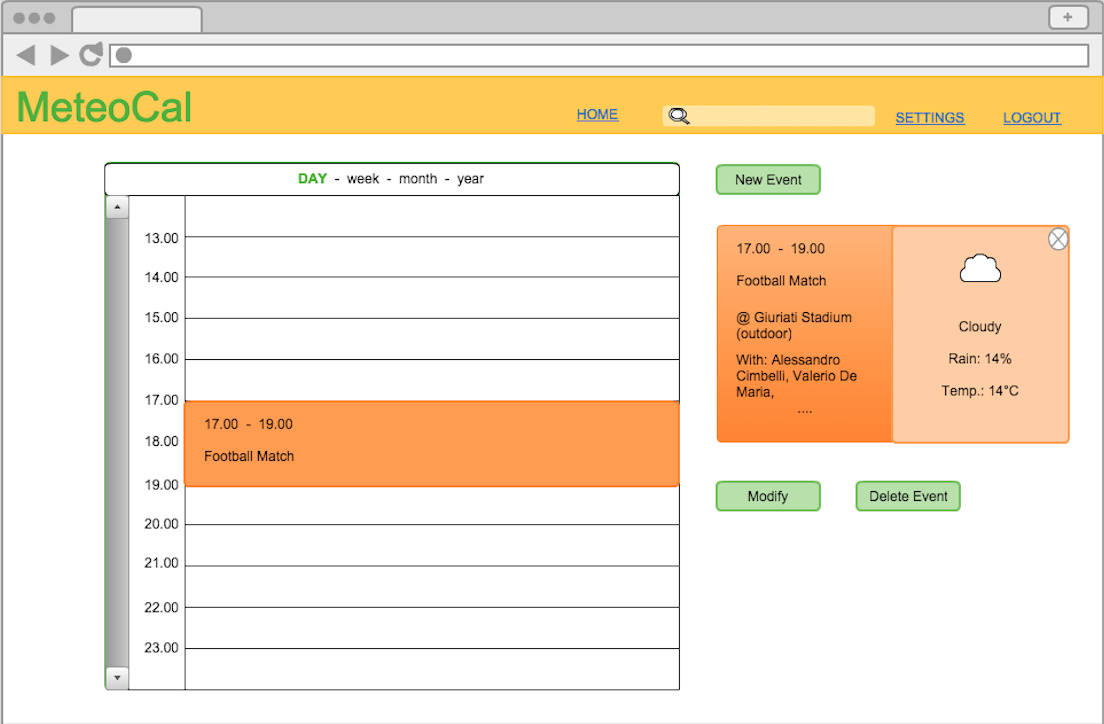
\includegraphics[width={\linewidth}]{./UI_mockups/04-registered_home.png}\vspace{3mm}

Where they can explore their calendar (on the left) and event details (on the right) by clicking on them on the calendar. They can also choose to create a new event or modify or delete an existing one.
If the user chooses to delete the selected event the system will ask for a confirmation.
If the user chooses to modify the selected event or create a new one the system will provide the following page:

\vspace{3mm}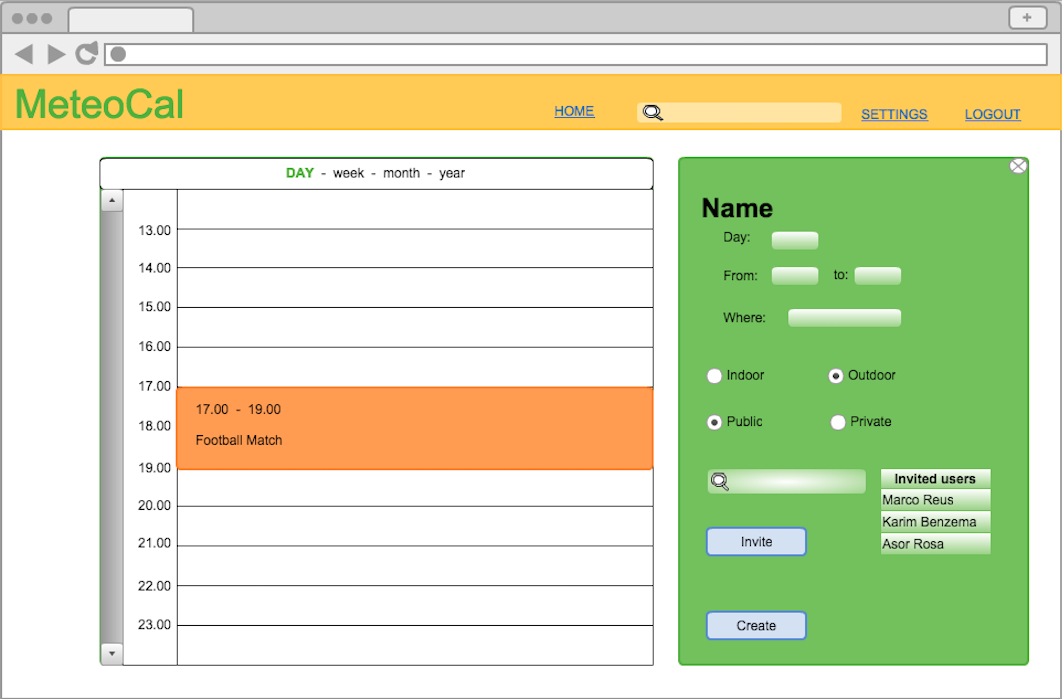
\includegraphics[width={\linewidth}]{./UI_mockups/05-create_event.png}\vspace{3mm}

Where he can submit the event details.
When the user logs into the system he receives the pending notifications (if any). This is the notification of an event invite:

\vspace{3mm}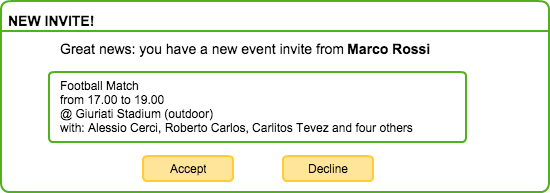
\includegraphics[width={\linewidth}]{./UI_mockups/06-invite_received.png}\vspace{3mm}

Where the user can see the event details and choose to accept or decline the invitation.
This is the notification of bad weather:

\vspace{3mm}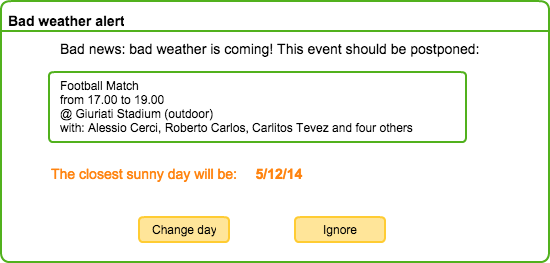
\includegraphics[width={\linewidth}]{./UI_mockups/07-bad_weather_three_days.png}\vspace{3mm}

This image is the one presented according to G8 (i.e. the one that proposes a different schedule three days in advance). The notification of G7 (a simple notification of bad weather) is similar except that it does not propose an alternative schedule:

\vspace{3mm}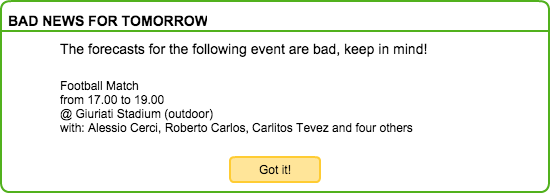
\includegraphics[width={\linewidth}]{./UI_mockups/11-bad_weather_one_day}\vspace{3mm}

From the “logged user homepage” the user can also search another user by his name and surname, then the system provides a list of possible matches:

\vspace{3mm}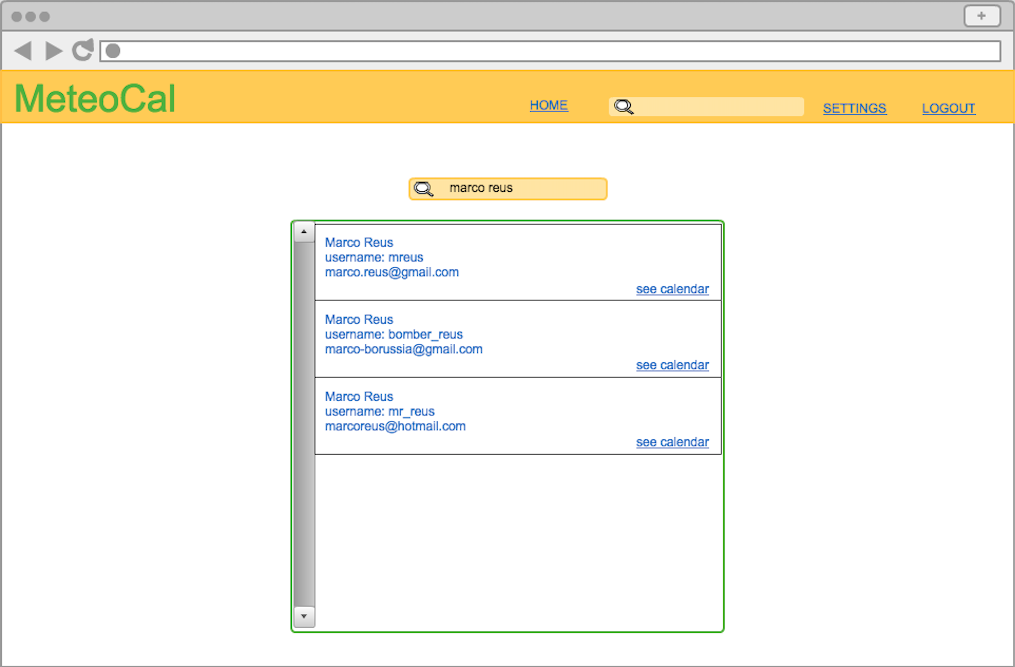
\includegraphics[width={\linewidth}]{./UI_mockups/08-search.png}\vspace{3mm}

Clicking on “see calendar” will bring the user to the following page:

\vspace{3mm}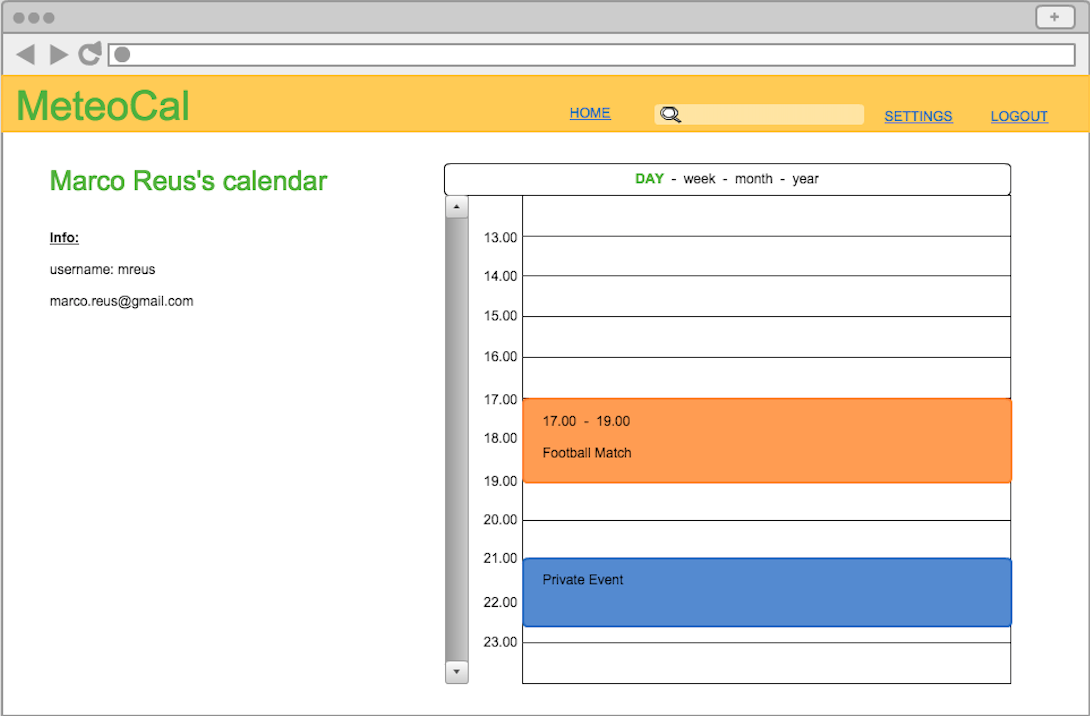
\includegraphics[width={\linewidth}]{./UI_mockups/09-other_calendar.png}\vspace{3mm}

Where the user can explore the schedule of the chosen user (if he has a public calendar). He will also be able to see public event details by clicking on them.
From the “logged user homepage” one can also click on “settings” and navigate to the following page:

\vspace{3mm}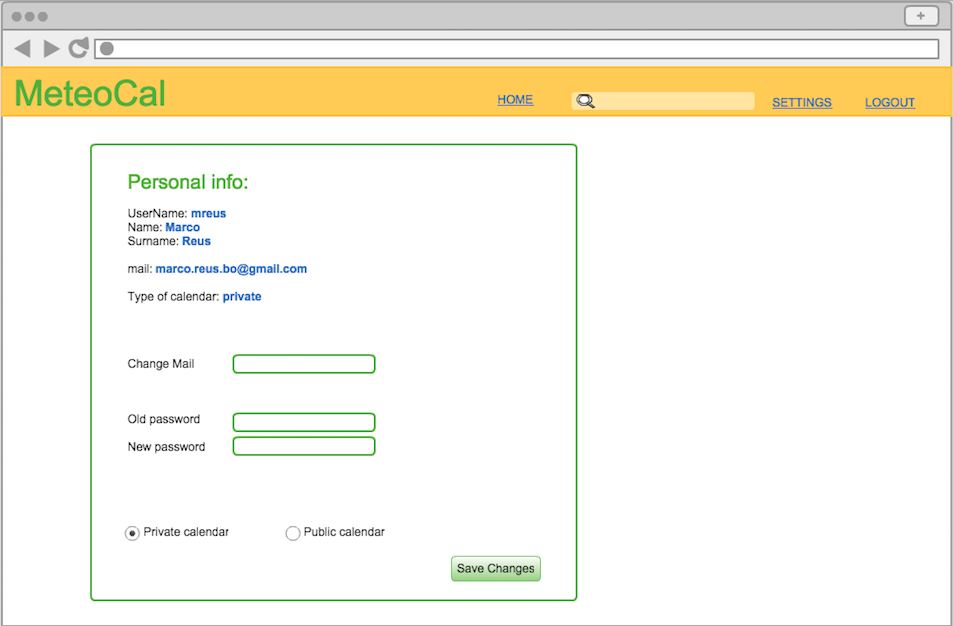
\includegraphics[width={\linewidth}]{./UI_mockups/10-settings.png}\vspace{3mm}

Where he can modify his data.
From all the pages, by clicking on “logout”, the user will log out of the system and return to the MeteoCal homepage.

\subsection{Hardware interfaces}
The software product does not provide any hardware interface.

\subsection{Software interfaces}

\subsubsection{Database management system}
\begin{itemize}
\item Name: MySQL
\item Mnemonic: MySQL
\item Specification number: Community Server
\item Version number: 5.6.21
\item Source: \url{http://dev.mysql.com/downloads/mysql/}
\end{itemize}

\subsubsection{Application server}
\begin{itemize}
\item Name: GlassFish Server
\item Mnemonic: GlassFishAS
\item Specification number: Open Source Edition
\item Version number: 4.1
\item Source: \url{https://glassfish.java.net/download.html}
\end{itemize}

\subsubsection{Operating system}
The software product will run on any operating system that supports the JVM and the DBMS and AS described above.

\subsection{Communication interfaces}
\begin{tabular}{|c|c|c|}
\hline Protocol & Port & Service \\ 
\hline TCP & 80 & World Wide Web \\ 
\hline TCP & 3306 & MySql (only if it is on a different physical server) \\ 
\hline 
\end{tabular}

\subsection{Memory}
The minimum memory requirements are:
\begin{itemize}
\item Primary memory:
\item Secondary memory:
\end{itemize}

\subsection{Operations}
A user can interact with the system as a functional user (unregistered or registered). For all the users, their functional operations are described in the product functions section.

\subsection{Site adaptation requirements}
The software product requires the following in order to run:
\begin{itemize}
\item JVM
\item AS
\item DBMS
\item Primary memory required space
\item Secondary memory required space
\end{itemize}
Users are required to have installed any of the following web browsers: IE6.0+, FF10+, Chrome 20+.

\section{Product functions}
This section provides a summary of the major functions of the software product.

\subsection{General requirements}
We have identified 3 main general requirements:
\begin{itemize}
\item Managing users
\item Managing calendars
\item Managing weather forecasts
\end{itemize}
The functional and non-functional requirements are defined and explained in detail in the following subsections.

\subsubsection{Managing users}
Functional requirements:
\begin{enumerate}[label = FR \arabic*:]
\item Register to system
\item Login
\item Logout
\item Modify password
\item Recover password
\item Update personal data
\end{enumerate}
Non-functional requirements:
\begin{enumerate}[label = NFR \arabic*:]
\item User password must be stored securely
\item System must support high number of users
\end{enumerate}

\subsubsection{Managing calendars}
Functional Requirements:
\begin{enumerate}[label = FR \arabic*:]
\item Add a new event
\item Modify an existing event
\item Delete an existing event
\item View your own schedule 
\item View the details of your own event
\item Send an invitation to other users
\item Reply to an invitation
\item See the schedule of other users if their calendar is public
\item See the details of other user's public events
\item Receive a notification when the event details changes
\end{enumerate}

\subsubsection{Managing weather forecasts}
Functional requirements:
\begin{enumerate}[label = FR \arabic*:]
\item Send a notification the day before an event in case of bad weather to all the event's participants
\item Propose an alternative schedule three days before an event in case of bad weather to the event creator
\item Show the weather forecasts for the scheduled events 
\end{enumerate}
Non-functional requirements:
\begin{enumerate}[label = NFR \arabic*:]
\item The displayed forecasts should be updated every XYZ time
\item The system has to interface with a Meteo service to collect forecasts
\end{enumerate}

\section{User characteristics}
Intended user should meet the following characteristics:
\begin{itemize}
\item Knowledge in using a browser
\end{itemize}

\section{Constraints}
The following constraints apply to the software product:

\subsection{Regulatory policies}
The software product does not have to meet any regulatory policies. 

\subsection{Hardware limitations}
The software product does not have any hardware limitations.

\subsection{Software limitations}
The system has to be developed using the Java EE platform. The business logic must be implemented using EJBs. 

\subsection{Interfaces to other applications}
The software product has to interface with one Meteorological service to get forecasts. 

\subsection{Parallel operation}
The system has to support simultaneous operation performed by different users. The most frequent situation to handle will be users simultaneously consulting and updating their own calendars. 

\subsection{Audit functions}
The software product does not perform any audit. 

\subsection{Control functions}
The software product does not control any device or any other system. 

\subsection{Higher-order language requirements}
The software product requires basic knowledge of HTML, Java and JEE technologies. 

\subsection{Signal handshake protocols}
The software product does not manage any handshake protocol. 

\subsection{Reliability requirements}
The software product does not require any specific requirements to perform and maintain its functions under normal operation. 

\subsection{Criticality of the application}
The software product requires proper support for concurrent users. 

\subsection{Safety and security considerations}
User data has to be stored and managed in a secure way.

\section{Assumptions and Dependencies}
The requirements in this document are grounded on the following assumptions:
\begin{itemize}
\item The JVM is already installed on the OS
\item Users have a decent and acceptable Internet connection.
\end{itemize}

\section{Apportioning of requirements}
Future releases of the software product may provide support for:
\begin{itemize}
\item Synchronization with other calendars
\item Multiple calendars
\item Avoid conflicting events
\item Periodical weather updates
\end{itemize}

\clearpage
\part{Specific Requirements}

\section{External interface requirements}

\subsection{User interfaces}
The storyboard in figure \ref{fig:Storyboard} describes the workflow to get from the login page to the exploration of the calendar of another user.
\begin{figure}[h!]
\centering
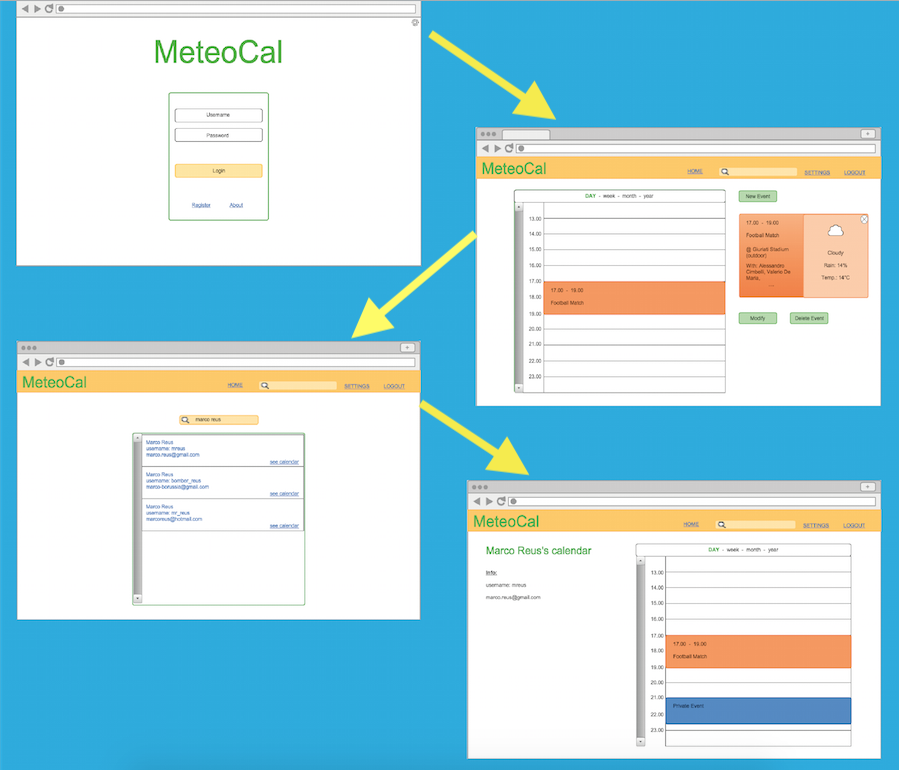
\includegraphics[width=\linewidth]{./UI_mockups/storyboard.png}
\caption[Storyboard]{Storyboard from login to another user's calendar}
\label{fig:Storyboard}
\end{figure}

\subsection{Hardware interfaces}
The software product does not provide any hardware interfaces.

\subsection{Software interfaces}
The software product does not provide any software interfaces.

\subsection{Communications interfaces}
The software product does not provide any communications interfaces.

\section{Functional Requirements}
\subsection{Scenarios}

\subsubsection{Registering in the system }
\begin{tabular}{| p{3cm} | p{10cm} |}
\hline \multicolumn{2}{|c|}{\textbf{Registering in the system }} \\ 
\hline Code        & SC001 \\ 
\hline Description & Describing how a user registers in the system \\
\hline Goal        & \begin{itemize}\item G1: Allow the registration of new users\end{itemize}\\
\hline Assumptions & \begin{enumerate} \item User is not registered \end{enumerate} \\
\hline \multicolumn{2}{|p{13cm}|}{Valerio wants to find a way to manage the schedule of his outdoor workouts, he asks a friend and becomes aware of the existence of MeteoCal. He navigates to the MeteoCal website and decides to register, so he clicks on "Register" button. The system provides him a form to be filled with mandatory information: his username, password, email address, name and surname. At the end he can press the “Save” button or the “Cancel” button. He saves and then logs out since he has to go out running.}\\
\hline
\end{tabular}

\subsubsection{User logs into the system}
\begin{tabular}{| p{3cm} | p{10cm} |}
\hline \multicolumn{2}{|c|}{\textbf{User logs into the system}} \\ 
\hline Code & SC002 \\ 
\hline Description & Describing how a user logs into the system \\
\hline Goal & \begin{itemize}\item G2: Allow users to view, create, update and delete events in their calendar\end{itemize}\\
\hline Assumptions & \begin{enumerate}
\item User is registered 
\item User correctly inserts the data
\end{enumerate} \\
\hline \multicolumn{2}{|p{13cm}|}{Valerio is back from his workout and wants to try his new calendar. He opens a web browser and navigates to the website of MeteoCal, where he clicks on a “Login” button. The system provides him a form where he inserts his username and his password, then he clicks on a “submit” button. Now he sees a page with his calendar. He is interrupted by a phone call.}\\
\hline
\end{tabular}

\subsubsection{User creates an event}
\begin{tabular}{| p{3cm} | p{10cm} |}
\hline \multicolumn{2}{|c|}{\textbf{User creates an event}} \\ 
\hline Code & SC003 \\ 
\hline Description & Describing how a user creates a new event\\
\hline Goal & \begin{itemize}\item G2: Allow users to view, create, update and delete events in their calendar\end{itemize}\\
\hline Assumptions & \begin{enumerate}
\item User is logged
\end{enumerate} \\
\hline \multicolumn{2}{|p{13cm}|}{Valerio finishes his phone call and returns to the MeteoCal website. He decides to schedule a running session for the next week: he clicks on an “Add event” button. The system provides a form where he is asked to provide a name for his appointment, a date, the starting and ending time. He is also asked to specify whether the event will take place outdoor or indoor. He specifies that it has to be a private event. Then he clicks on a “Save event” button and closes the website.}\\
\hline
\end{tabular}

\subsubsection{User modifies an event}
\begin{tabular}{| p{3cm} | p{10cm} |}
\hline \multicolumn{2}{|c|}{\textbf{User modifies an event}} \\ 
\hline Code & SC004 \\ 
\hline Description & Describing how a user modifies an existing event \\
\hline Goal & \begin{itemize}\item G2: Allow users to view, create, update and delete events in their calendar\end{itemize}\\
\hline Assumptions & \begin{enumerate}
\item User is logged
\item User has at least one event in his calendar
\end{enumerate} \\
\hline \multicolumn{2}{|p{13cm}|}{Valerio suddenly realizes that he scheduled the workout on a wrong day, so he goes back to the MeteoCal website and logs into the system. The system provides him a calendar where he can sees his appointments, he clicks on the interesting event and appears a description of the event and two buttons: “modify” and “delete”. He clicks on “modify” and the system provides a form with the data of the event, he modifies the day and clicks “save”. Now on the calendar the event is scheduled on the new date.}\\
\hline
\end{tabular}

\subsubsection{User views his calendar}
\begin{tabular}{| p{3cm} | p{10cm} |}
\hline \multicolumn{2}{|c|}{\textbf{User views his calendar}} \\ 
\hline Code & SC005 \\ 
\hline Description & Describing how a user views the details of his appointments \\
\hline Goal & \begin{itemize}\item G2: Allow users to view, create, update and delete events in their calendar\end{itemize}\\
\hline Assumptions & \begin{enumerate}
\item User is logged
\item User has at least one event in his calendar
\end{enumerate} \\
\hline \multicolumn{2}{|p{13cm}|}{Valerio forgot when he has to run, so he decides to check on MeteoCal. After the login the system provides an overview of his calendar, with a visual representations of his appointments, he clicks on the desired activity and the system visualize the details of the event: when it is scheduled, where it will take place (the place and if it's indoor or/outdoor) and the invited users. The systems also shows the forecast for the selected event.}\\
\hline
\end{tabular}

\subsubsection{User deletes an event}
\begin{tabular}{| p{3cm} | p{10cm} |}
\hline \multicolumn{2}{|c|}{\textbf{User deletes an event}} \\ 
\hline Code & SC006 \\ 
\hline Description & Describing how a user deletes an existing event \\
\hline Goal & \begin{itemize}\item G2: Allow users to view, create, update and delete events in their calendar\end{itemize}\\
\hline Assumptions & \begin{enumerate}
\item User is logged
\item User has at least one event in his calendar
\end{enumerate} \\
\hline \multicolumn{2}{|p{13cm}|}{Valerio broke a leg during his last workout, so he decides to remove the scheduled running from MeteoCal. From his homepage (after the log in) he clicks on the event and from the new page he clicks on a “delete” button, the system asks for a confirmation, and after the confirm the event disappears from the calendar.}\\
\hline
\end{tabular}

\subsubsection{User invites another user to his event}
\begin{tabular}{| p{3cm} | p{10cm} |}
\hline \multicolumn{2}{|c|}{\textbf{User invites another user to his event}} \\ 
\hline Code & SC007 \\ 
\hline Description & Describing how a user invites another user to his event \\
\hline Goal & \begin{itemize}\item G3: Allow users to invite other users to their events \end{itemize}\\
\hline Assumptions & \begin{enumerate}
\item User is logged
\item User is visualizing the details of one of his events
\item User doesn't try to invite himself
\item User correctly inserts the name of the other user
\end{enumerate} \\
\hline \multicolumn{2}{|p{13cm}|}{While visualizing the details of his scheduled running workout Valerio has a great idea: inviting to the workout his friend Ilario. Valerio clicks on an “Invite” button and the system provides a form where he can insert the username of the desired user, he inserts the username of his friend and clicks on a “Send invitation” button. While waiting for the answer he sends an sms to his friend.}\\
\hline
\end{tabular}

\subsubsection{Invited user accepts}
\begin{tabular}{| p{3cm} | p{10cm} |}
\hline \multicolumn{2}{|c|}{\textbf{Invited user accepts}} \\ 
\hline Code & SC008 \\ 
\hline Description & Describing how a user accepts an invitation \\
\hline Goal & \begin{itemize}\item G4: Allow invited users to either accept or decline the invitation \end{itemize}\\
\hline Assumptions & \begin{enumerate}
\item User is registered
\item User has received an invite
\item User has not logged to system since he has received the invite
\end{enumerate} \\
\hline \multicolumn{2}{|p{13cm}|}{Ilario is a friend of Valerio and is a new user of MeteoCal. He receives a sms by Valerio and decides to check if he has received the event invitation. He logs into MeteoCal and the system presents him a notification of the invitation where he can see the event details. Since he likes the idea, he clicks on an “Accept” button. The event appears on his calendar.}\\
\hline
\end{tabular}

\subsubsection{User declines an event invite}
\begin{tabular}{| p{3cm} | p{10cm} |}
\hline \multicolumn{2}{|c|}{\textbf{User declines an event invite}} \\ 
\hline Code & SC009 \\ 
\hline Description & Describing how a user declines an event invite. \\
\hline Goal & \begin{itemize}\item G4: Allow invited users to either accept or decline the invitation\end{itemize}\\
\hline Assumptions & \begin{enumerate}
\item The user is registered
\item The user has been invited to another user's event
\end{enumerate} \\
\hline \multicolumn{2}{|p{13cm}|}{Valerio has just returned home after a long training session. After a shower, he turns on his computer to check what are his appointments for the following day. In order to do so he opens the browser, navigate to the MeteoCal website and login into the system. Valerio starts to browse his events when an invite notification appears in the middle of the page. Leonardo, his south-american friend, invited him to try a Samba lesson later in the evening, at 21.30. Valerio feels very tired because of his training so he clicks on the “decline” button. The notification disappears and Valerio finishes to check his appointments.}\\
\hline
\end{tabular}

\subsubsection{User search the calendar of another user }
\begin{tabular}{| p{3cm} | p{10cm} |}
\hline \multicolumn{2}{|c|}{\textbf{User search the calendar of another user }} \\ 
\hline Code & SC010 \\ 
\hline Description & Describing how a user can search the calendar of another user.\\
\hline Goal & \begin{itemize}\item G5: Allow users to see other users public calendar\end{itemize}\\
\hline Assumptions & \begin{enumerate}
\item Both user are registered
\item The second user's calendar is public
\end{enumerate} \\
\hline \multicolumn{2}{|p{13cm}|}{Valerio has changed his mind and he decided that he wants to take a dance lesson with Leonardo. Unfortunately it’s already 21.45 and the lesson is already started. Valerio decides to check whether Leonardo will go to other lessons during the week. He opens his MeteoCal homepage, writes Leonardo Tanque (his friend’s name) in the search bar in the top right and press enter. He could have used also Leonardo’s username but, at the moment, it didn’t come to his mind. After performing the search the system shows a page displaying all the results. There are a lot of users called Leonardo Tanque. Valerio scrolls down the bar on the left until he finds his friend by recognizing his email address (which is displayed along with the name and the userName). Valerio clicks on the “see calendar” link on the right of the result and gets to Leonardo’s calendar.}\\
\hline
\end{tabular}

\subsubsection{A user looks through the calendar of another user}
\begin{tabular}{| p{3cm} | p{10cm} |}
\hline \multicolumn{2}{|c|}{\textbf{A user looks through the calendar of another user}} \\ 
\hline Code & SC011 \\ 
\hline Description & Describing how a user navigate through another user's calendar\\
\hline Goal & \begin{itemize}\item G5: Allow users to see other users public calendar\item G6: Allow users to see other users public events details\end{itemize}\\
\hline Assumptions & \begin{enumerate}
\item Both user are registered
\item The second user's calendar is public
\end{enumerate} \\
\hline \multicolumn{2}{|p{13cm}|}{Valerio has reached Leonardo’s calendar. He selects the week view. Leonardo has some events programmed for next Wednesday. He has a private event going from 13.00 to 15.00 and a public event called “Samba” going from 21.30 to 22.30. The calendar shows only public events name. Valerio wants to be sure that “Samba” is a dance lesson so he clicks on the event to get further details. The event is public so a window showing all the event information appears on the right. Valerio sees that it will take place indoor in the “Samba dance school” so he has just found what he was looking for. Now he’s quite curious about what Leonardo has to do from 13.00 to 15.00. He tries to see the details but the event is private and, when he clicks on it, nothing happens.}\\
\hline
\end{tabular}

\subsubsection{The user receives the bad weather alert}
\begin{tabular}{| p{3cm} | p{10cm} |}
\hline \multicolumn{2}{|c|}{\textbf{The user receives the bad weather alert}} \\ 
\hline Code & SC012 \\ 
\hline Description & After entering MeteoCal the user receives a bad weather alert with one day of advance from the event\\
\hline Goal & \begin{itemize}\item G7: Send a notification to all the participants one day in advance in case a bad weather\end{itemize}\\
\hline Assumptions & \begin{enumerate}
\item The user is registered
\item The user is going to take part in an outdoor event on the following day
\item The weather forecasts for the following day are bad.
\end{enumerate} \\
\hline \multicolumn{2}{|p{13cm}|}{It’s Friday and Valerio decides to check his programs for the weekend. His friend Guglielmo invited him to a trekking trip on the mountains near Como. Valerio is worried about the weather conditions, he heard  that it might rain. He logins and, as soon as he gets to his homepage, a notification appears. It warns Valerio that the weather forecasts for the trip (planned for the next day) are bad. There’s a high chance of rain. Thus Valerio will put a raincoat in his rucksack.}\\
\hline
\end{tabular}

\subsubsection{The system propose a sunny day to the user}
\begin{tabular}{| p{3cm} | p{10cm} |}
\hline \multicolumn{2}{|c|}{\textbf{The system propose a sunny day to the user}} \\ 
\hline Code & SC013 \\ 
\hline Description & If three days before the event its weather forecasts are bad, the system warns the creator and suggests to him to change the date to the closest sunny day. The user can move the event or leave it on the scheduled day.\\
\hline Goal & \begin{itemize}\item G8: Propose an alternative schedule to the event creator three day in advance in case of bad weather\end{itemize}\\
\hline Assumptions  & \begin{enumerate}
\item The user is registered
\item The user created an event
\item There are bad weather forecasts for the event
\item The event will take place after three days
\end{enumerate} \\
\hline \multicolumn{2}{|p{13cm}|}{Valerio planned a trip to the seaside with his friend Alessandro and created the related event on MeteoCal. Three days before the event Valerio wants to check whether he invited his friend to the event or not. He logins in MeteoCal and, as soon as he enters the homepage, a notification appears. It says that the  weather forecasts for the seaside trip are bad. It also points out that the closest sunny day will be Wednesday. Valerio can ignore the message (“ignore” button) or move the event to Wednesday (“move” button). He thinks about it and finally he decides to click on the move button. The event is postponed and scheduled for Wednesday, the other event details (time, place ecc..) remain the same.}\\
\hline
\end{tabular}

\subsubsection{A user gets notified that an event date has been changed}
\begin{tabular}{| p{3cm} | p{10cm} |}
\hline \multicolumn{2}{|c|}{\textbf{A user gets notified that an event date has been changed}} \\ 
\hline Code & SC014 \\ 
\hline Description & When the creator of an event changes its details all the participants (but not the creator) are notified.\\
\hline Goal & G9: Notify all the event's participant in case the creator changes some details\\
\hline Assumptions  & \begin{enumerate}
\item The user is registered
\item He accepted the invite to an event
\item The creator changed the date of the event for bad weather conditions.
\end{enumerate} \\
\hline \multicolumn{2}{|p{13cm}|}{Alessandro wants to check the leaving time for his trip to the seaside with Valerio. He logins and access his MeteoCal homepage. While browsing through his events he gets a notification.  It states that Valerio (the event creator) chanced the date of the seaside trip. The event is now planned for Wednesday. Alessandro returns to his calendar page.}\\
\hline
\end{tabular}

\subsubsection{A user changes his data}
\begin{tabular}{| p{3cm} | p{10cm} |}
\hline \multicolumn{2}{|c|}{\textbf{A user changes his data}} \\ 
\hline Code & SC015 \\ 
\hline Description & A user accesses his settings page and change his password and his email address.\\
\hline Goal & G10: Allow users to modify their data\\
\hline Assumptions  & \begin{enumerate}
\item The user is registered
\item The user types a valid email account and the right old password
\end{enumerate} \\
\hline \multicolumn{2}{|p{13cm}|}{Valerio has just created a new email account on gmail. He decides that he wants to use it in MeteoCal instead of his previous email address. He logs into the system and gets to his homepage. He clicks on the settings button on the top right of the page. The settings page shows his personal details. He enters his new email in the appropriate box. Valerio wants to be sure that his private events are safe so he decides to change the password. He types in the appropriate boxes his old password and the new one. Finally Valerio presses the save button. His information are updated by system and the settings page is changed consequently. }\\
\hline
\end{tabular}

\subsubsection{The system updates the meteo forecasts}
\begin{tabular}{| p{3cm} | p{10cm} |}
\hline \multicolumn{2}{|c|}{\textbf{The system updates the meteo forecasts}} \\ 
\hline Code & SC016 \\ 
\hline Description & MeteoCal asks an external meteo service for updated weather forecasts for all the scheduled events. \\
\hline Goal & \begin{itemize}
\item G7: Send a notification to all the participants one day in advance in case of bad weather
\item G8: Propose an alternative schedule to the event creator three day in advance in case of bad weather.
\end{itemize}\\
\hline Assumptions  & \begin{enumerate}
\item The systems has some user events in his database
\item The system has an interface to “speak” with an external weather forecasts service
\end{enumerate} \\
\hline \multicolumn{2}{|p{13cm}|}{The system has to update the weather forecasts of some outdoor events because they’re obsolete (they haven’t been updated for more than one day). To do so MeteoCal ask an external service for the forecasts that he needs and waits for the each answer. When the external service answers the systems updates the events. Users are now  able to see the up to date forecasts for their events.}\\
\hline
\end{tabular}

\section{Analysis model}
The analysis model represents the core concepts; the diagram in figure \ref{fig:ClassDiag} introduces the conceptual classes that we have decided to include in the software product.
\begin{figure}[h]
\centering
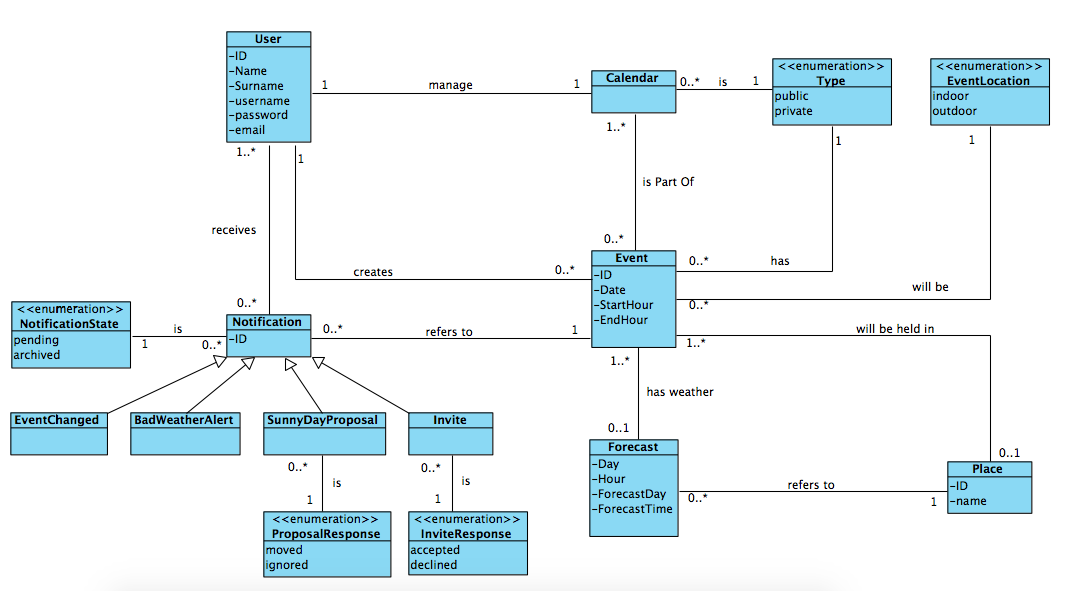
\includegraphics[width=\linewidth]{./Uml/ClassDiagram.png}
\caption[ClassDiag]{Class diagram}
\label{fig:ClassDiag}
\end{figure}

\section{State chart model}
The following diagrams represents the evolution of some objects in our system.

Figure \ref{fig:InviteStateChart} depicts the evolution of the notification of an event invite.
\begin{figure}[h!]
\centering
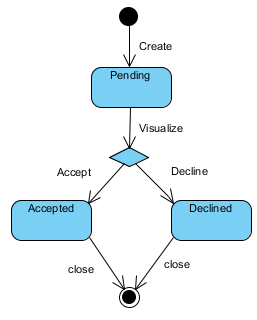
\includegraphics[height=7cm]{./Uml/StateDiagram_invite.png}
\caption[InviteStateChart]{Invite notification state chart}
\label{fig:InviteStateChart}
\end{figure}

Figure \ref{fig:3DayStateChart} depicts the evolution of the notification sent to the event creator to propose an alternative schedule.
\begin{figure}[h!]
\centering
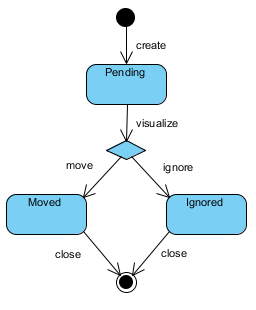
\includegraphics[height=7cm]{./Uml/StateDiagram_3day.png}
\caption[3DayStateChart]{New schedule proposal state chart}
\label{fig:3DayStateChart}
\end{figure}

Figure \ref{fig:badWeatherStateChart} depicts the evolution of the notification of bad weather sent to all the event's participants one day in advance. It also describes a notification sent when the event details are changed.
\begin{figure}[h!]
\centering
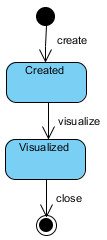
\includegraphics[height=5cm]{./Uml/StateDiagram_badWeather_eventChanged.png}
\caption[BadWeatherStateChart]{Bad weather and event changed notification state chart}
\label{fig:badWeatherStateChart}
\end{figure}

\section{Activity Model}
Since the main goal of the software product is to create new event, in figure \ref{fig:ActivityDiag} we introduce the activity model of the creation of a new event.
\begin{figure}[h!]
\centering
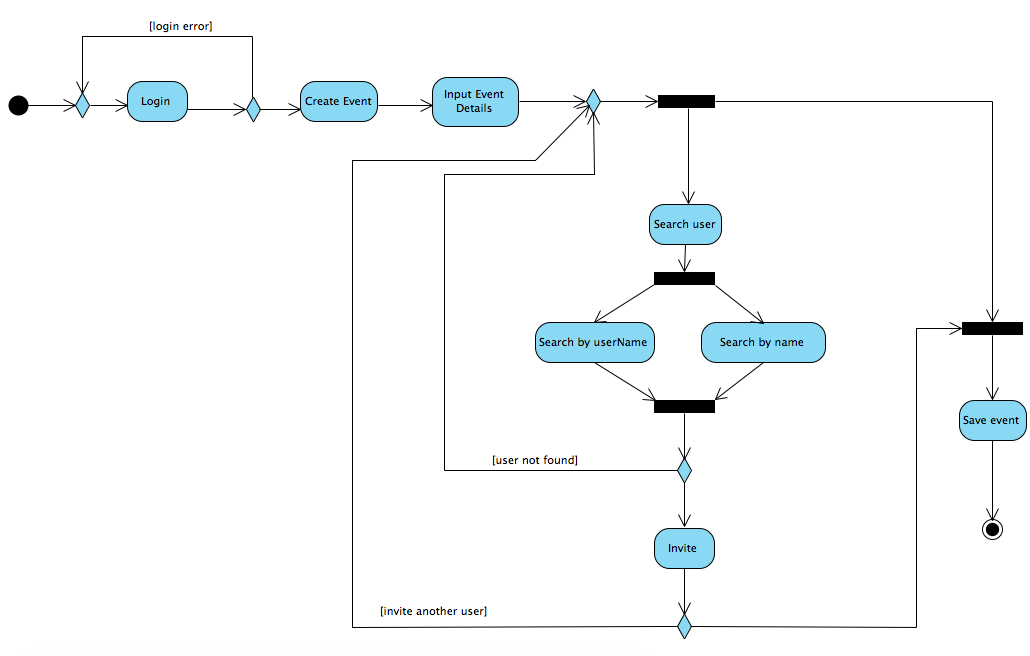
\includegraphics[height=7cm]{./Uml/ActivityDiagram.png}
\caption[ActivityDiag]{Event creation activity diagram}
\label{fig:ActivityDiag}
\end{figure}

\section{Use case model}
Below we separately present the use cases associated with our two actors:
\begin{itemize}
\item Unlogged user
\item Logged user
\end{itemize}


\subsection{Unlogged User}
Figure \ref{fig:Unlogged_usc} depicts the use cases of an unlogged user.
\begin{figure}[h]
\centering
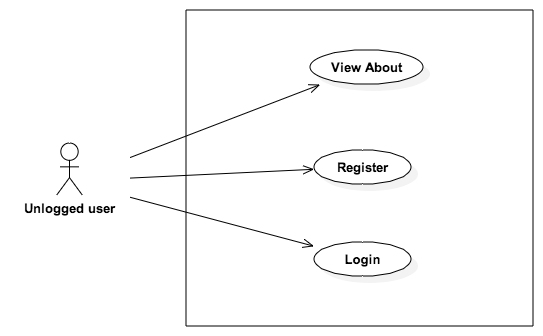
\includegraphics[width=\linewidth]{./Use_case/unlogged_usecase.png}
\caption[Unlogged_usc]{Unlogged user use case}
\label{fig:Unlogged_usc}
\end{figure}

\clearpage
\subsubsection{User register to the system}

\begin{tabular}[h]{| p{3cm} | p{10cm} |}
\hline \multicolumn{2}{|c|}{\textbf{User register to the system}} \\ 
\hline Code & USC001 \\ 
\hline Description & Describing how unregistered users can register to the system\\
\hline Goal & G1: Allow the registration of new users \\
\hline Assumptions  & \begin{enumerate}
\item The user is not registered to the system
\end{enumerate} \\
\hline Actors &  \begin{enumerate}
\item The unregistered user
\end{enumerate} \\
\hline Entry condition & The unregistered user navigates to the register page \\
\hline Exit condition & User data are correctly saved a confirmation is displayed\\
\hline Flow of events & \begin{enumerate}
\item The unregistered user navigates to the MeteoCal registering page
\item The system provides a form to be filled with Username, Name, Surname, Mail, Password
\item The unregistered user fills the form and clicks “Ready”
\item The system saves the new user data and display a confirmation window
\end{enumerate}\\
\hline Exceptions & \begin{itemize}
\item If some data are missing the system shows an error
\item If the username or the password have already been used by another user the system shows an error 
\end{itemize} \\
\hline Special requirements & \\
\hline Nonfunctional requirements & \\
\hline
\end{tabular}
\begin{figure}[h]
\centering
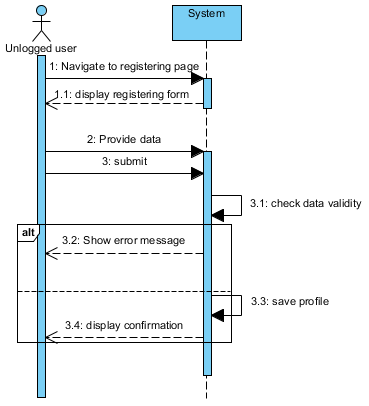
\includegraphics[width=\linewidth]{./Sequence_diag/USC001.png}
\caption[USC001]{USC001 - User register to the system}
\label{fig:USC001}
\end{figure}

\clearpage
\subsubsection{A registered user logs into the system}

\begin{tabular}[h]{| p{3cm} | p{10cm} |}
\hline \multicolumn{2}{|c|}{\textbf{A registered user logs into the system}} \\ 
\hline Code & USC002 \\ 
\hline Description & Describing how a registered user logs into the system \\
\hline Goal & G1: Allow users to create update and delete events in their calendar \\
\hline Assumptions  & \begin{enumerate}
\item User is registered to the system
\item User is not logged to the system
\end{enumerate} \\
\hline Actors &  \begin{enumerate}
\item The registered user
\end{enumerate} \\
\hline Entry condition & The user navigates to the MeteoCal homepage\\
\hline Exit condition & The user is logged into the system \\
\hline Flow of events & \begin{enumerate}
\item The registered user navigates to the MeteoCal homepage
\item The system provides a form to be filled with username and password
\item The user inserts his data and clicks login
\item The system logs the user and redirect the user to the “Registered user homepage”
\end{enumerate}\\
\hline Exceptions & If the inserted data are not correct the system shows an error message \\
\hline Special requirements & \\
\hline Nonfunctional requirements &  \\
\hline
\end{tabular}
\begin{figure}[h]
\centering
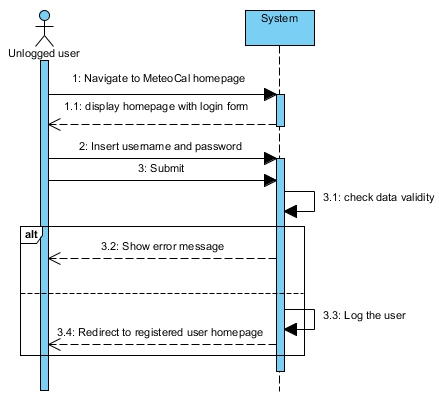
\includegraphics[width=\linewidth]{./Sequence_diag/USC002.png}
\caption[USC002]{USC002 - A registered user logs into the system}
\label{fig:USC002}
\end{figure}

\clearpage
\subsection{Logged User}
Figure \ref{fig:Logged_usc_simple} contains the simplified version of the logged user use case, while figure \ref{fig:Logged_usc} depicts the complete one.

\begin{figure}[h!]
\centering
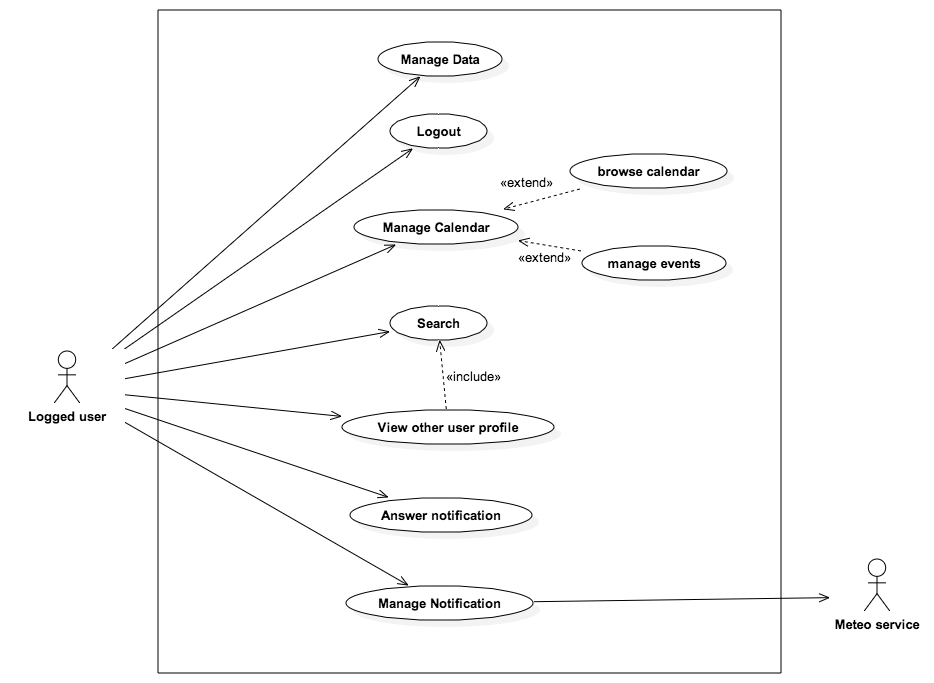
\includegraphics[width=\linewidth]{./Use_case/logged_usecase_simple.png}
\caption[Logged_usc_simple]{Logged user use case. Simplified}
\label{fig:Logged_usc_simple}
\end{figure}

\begin{figure}[h!]
\centering
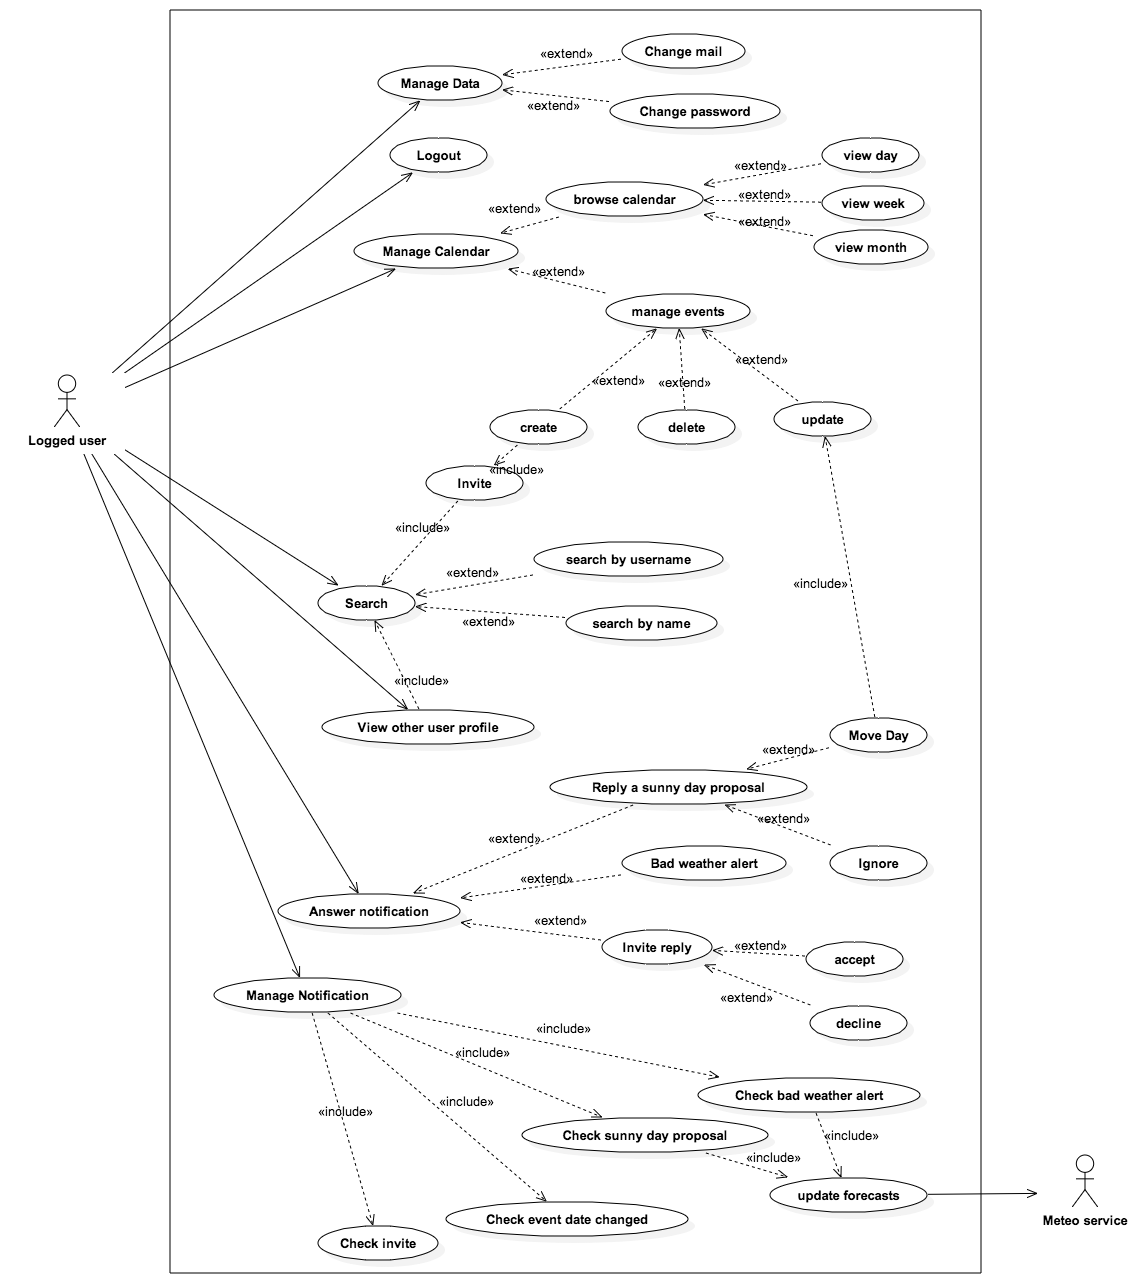
\includegraphics[width=16cm]{./Use_case/logged_usecase.png}
\caption[Logged_usc]{Logged user use case}
\label{fig:Logged_usc}
\end{figure}

\clearpage
\subsubsection{Logged user creates a new event}

\begin{tabular}[h]{| p{3cm} | p{10cm} |}
\hline \multicolumn{2}{|c|}{\textbf{Logged user creates a new event}} \\ 
\hline Code & USC003 \\ 
\hline Description & Describing how a logged user can create new events \\
\hline Goal & G2: Allow users to view, create, update and delete events in their calendar\\
\hline Assumptions  & \begin{enumerate}
\item User is logged
\item User is visualizing the “registered user homepage”
\end{enumerate} \\
\hline Actors &  \begin{enumerate}
\item The logged user
\end{enumerate} \\
\hline Entry condition & The user clicks on “New event” \\
\hline Exit condition & The event is created \\
\hline Flow of events & \begin{enumerate}
\item The user clicks on “New event”
\item The system provides a form to be filled with the event data (Day, From, To, Where, Indoor/Outdoor, Public/Private and a possibly empty list of invited users)
\item The user fills the form and clicks on “Create”
\item The system saves the event and shows a confirmation
\end{enumerate}\\
\hline Exceptions & If some data is missing the system shows an error \\
\hline Special requirements &  \\
\hline Nonfunctional requirements &  \\
\hline
\end{tabular}
\begin{figure}[h]
\centering
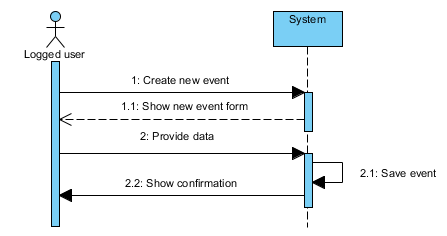
\includegraphics[width=\linewidth]{./Sequence_diag/USC003.png}
\caption[USC003]{USC003 - Logged user creates a new event}
\label{fig:USC003}
\end{figure}

\clearpage
\subsubsection{Logged user modifies an existing event}

\begin{tabular}[h]{| p{3cm} | p{10cm} |}
\hline \multicolumn{2}{|c|}{\textbf{Logged user modifies an existing event}} \\ 
\hline Code & USC004 \\ 
\hline Description & Describing how a logged user can modify the data of an event that he have created previously \\
\hline Goal & G2: \\
\hline Assumptions  & \begin{enumerate}
\item The user is logged
\item The user tries to modify an event that he have created before
\end{enumerate} \\
\hline Actors &  \begin{enumerate}
\item The logged user
\end{enumerate} \\
\hline Entry condition & From the “registered user homepage” the user selects an event and clicks on “Modify” \\
\hline Exit condition & The system modifies the event data and show a confirmation \\
\hline Flow of events & \begin{enumerate}
\item From his “registered user homepage” the user selects an event
\item The system displays the selected events data and a “Modify” button
\item The user clicks on “Modify”
\item The system provides a form with the old data
\item The user modifies the data and clicks “Save”
\item The system modifies the event data and show a confirmation
\end{enumerate}\\
\hline Exceptions & If some data are missing the system shows an error \\
\hline Special requirements & \\
\hline Nonfunctional requirements &  \\
\hline
\end{tabular}
\begin{figure}[h]
\centering
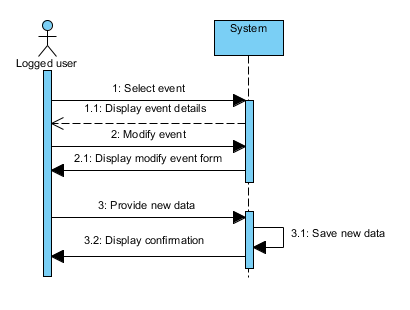
\includegraphics[width=\linewidth]{./Sequence_diag/USC004.png}
\caption[USC004]{USC004 - Logged user modifies an existing event}
\label{fig:USC004}
\end{figure}

\clearpage
\subsubsection{Logged user views the details of his events}

\begin{tabular}[h]{| p{3cm} | p{10cm} |}
\hline \multicolumn{2}{|c|}{\textbf{ Logged user views the details of his events }} \\ 
\hline Code & USC005 \\ 
\hline Description & Describing how a logged user can view his calendar and event details\\
\hline Goal & G2: Allow users to view, create, update and delete events in their calendar\\
\hline Assumptions  & \begin{enumerate}
\item User is logged
\item User has at least one event in his calendar
\end{enumerate} \\
\hline Actors &  \begin{enumerate}
\item The logged user
\end{enumerate} \\
\hline Entry condition & The user reaches the “registered user homepage” \\
\hline Exit condition & The user clicks on “X” \\
\hline Flow of events & \begin{enumerate}
\item The user reaches his “registered user homepage”
\item The system shows him a representation of his event, showing the name and the schedule of events
\item The user clicks on an event
\item The system shows him the event details: Starting and ending time, name, place, invited users and weather forecast
\item The user closes the event details by clicking on an “X”
\end{enumerate}\\
\hline Exceptions & \\
\hline Special requirements & \\
\hline Nonfunctional requirements & \\
\hline
\end{tabular}
\begin{figure}[h]
\centering
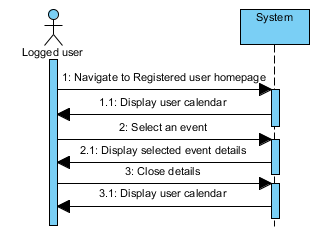
\includegraphics[width=\linewidth]{./Sequence_diag/USC005.png}
\caption[USC005]{USC005 - Logged user views the details of his events}
\label{fig:USC005}
\end{figure}

\clearpage
\subsubsection{Logged user deletes an event}

\begin{tabular}[h]{| p{3cm} | p{10cm} |}
\hline \multicolumn{2}{|c|}{\textbf{Logged user deletes an event}} \\ 
\hline Code & USC006 \\ 
\hline Description & Describing how a logged user removes an appointment from his calendar \\
\hline Goal & G2: Allow users to view, create, update and delete events in their calendar\\
\hline Assumptions  & \begin{enumerate}
\item User is logged and visualizing the details of one event in his calendar
\item User has at least one event in his calendar
\end{enumerate} \\
\hline Actors &  \begin{enumerate}
\item The logged user
\end{enumerate} \\
\hline Entry condition & The user clicks on “delete event” \\
\hline Exit condition & The system removes the appointment from the user’s calendar \\
\hline Flow of events & \begin{enumerate}
\item While visualizing the details of an event the user clicks on “delete event”
\item The system removes the appointment from the user’s calendar. If the user created the event and there are other users invited the system removes the event also from their calendars. If another user created the event and the current user is only a guest the system removes the event only from the current user’s calendar.
\end{enumerate}\\
\hline Exceptions & \\
\hline Special requirements & \\
\hline Nonfunctional requirements & \\
\hline
\end{tabular}
\begin{figure}[h]
\centering
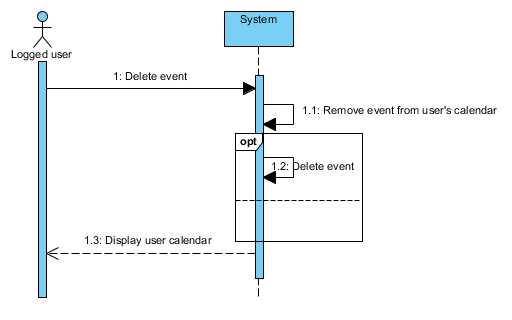
\includegraphics[width=\linewidth]{./Sequence_diag/USC006.png}
\caption[USC006]{USC006 - Logged user deletes an event}
\label{fig:USC006}
\end{figure}

\clearpage
\subsubsection{Logged user invites another user to his event}

\begin{tabular}[h]{| p{3cm} | p{10cm} |}
\hline \multicolumn{2}{|c|}{\textbf{ Logged user invites another user to his event }} \\ 
\hline Code & USC007 \\ 
\hline Description & Describing how a logged user can invite another user to his events \\
\hline Goal & G3: Allow users to invite other users to their events \\
\hline Assumptions  & \begin{enumerate}
\item User is logged and modifying the details of one of his events
\item User has at least one event in his calendar
\end{enumerate} \\
\hline Actors &  \begin{enumerate}
\item The logged user
\end{enumerate} \\
\hline Entry condition & User starts typying in an “invite” textbox \\
\hline Exit condition & The system sends an invite notification  and shows a confirmation\\
\hline Flow of events & \begin{enumerate}
\item The user starts typing in an “invite” textbox
\item The system searches for an user that matches the typed text by username, name, surname or e-mail and proposes a list of possible matches.
\item The user selects an user and clicks on “invite”
\item The system saves the invitation and shows a confirmation
\end{enumerate}\\
\hline Exceptions & If there are no possible matches the system shows an error \\
\hline Special requirements & \\
\hline Nonfunctional requirements & \\
\hline
\end{tabular}
\begin{figure}[h]
\centering
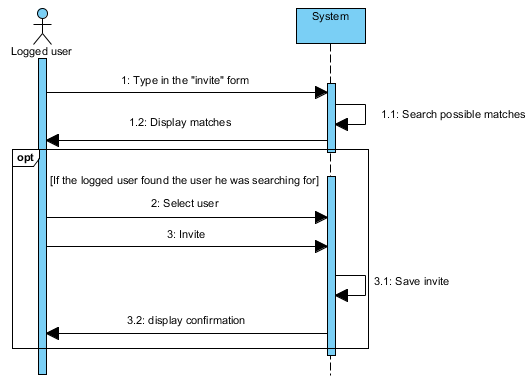
\includegraphics[width=\linewidth]{./Sequence_diag/USC007.png}
\caption[USC007]{USC007 - Logged user invites another user to his event}
\label{fig:USC007}
\end{figure}

\clearpage
\subsubsection{Registered user accepts an invitation}

\begin{tabular}[h]{| p{3cm} | p{10cm} |}
\hline \multicolumn{2}{|c|}{\textbf{ Registered user accepts an invitation }} \\ 
\hline Code & USC008 \\ 
\hline Description & Describing how a registered user receives the notification of an invite and accepts it \\
\hline Goal & G4: Allow invited users to either accept or decline the invitation \\
\hline Assumptions  & \begin{enumerate}
\item User is registered
\item User has received an invite
\item User has not logged to system since he has received the invite
\item The user accepts the invitation
\end{enumerate} \\
\hline Actors &  \begin{enumerate}
\item Registered user
\end{enumerate} \\
\hline Entry condition & User logs into the system \\
\hline Exit condition & System adds the user to the list of event’s participants\\
\hline Flow of events & \begin{enumerate}
\item The registered user logs into the system
\item The system notifies him that he has received an invitation. It shows the event creator’s name and surname, the event name, when and where it will take place and the event’s participants.
\item The user clicks on “Accept”
\item The system add the event to the user’s calendar an the user to the event’s participants.
\end{enumerate}\\
\hline Exceptions & \\
\hline Special requirements & \\
\hline Nonfunctional requirements & \\
\hline
\end{tabular}
\begin{figure}[h]
\centering
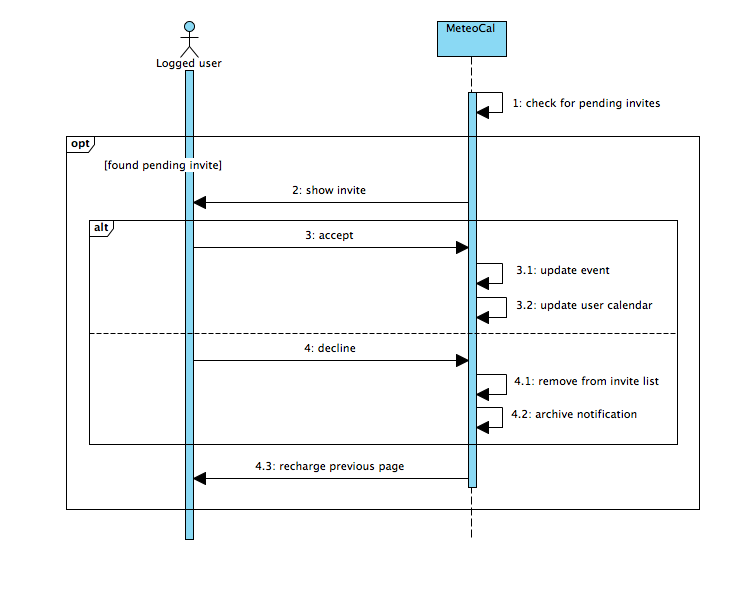
\includegraphics[width=\linewidth]{./Sequence_diag/USC008.png}
\caption[USC008]{USC008 - Registered user accepts an invitation}
\label{fig:USC008}
\end{figure}

\clearpage
\subsubsection{Decline an event invite}

\begin{tabular}[h]{| p{3cm} | p{10cm} |}
\hline \multicolumn{2}{|c|}{\textbf{Decline an event invite}} \\ 
\hline Code & USC009 \\ 
\hline Description & A user declines an event invite from another user \\
\hline Goal & G3: Allow invited users to either accept or decline the invitation\\
\hline Assumptions  & \begin{enumerate}
\item the user is registered
\item the user has been invited to another user's event
\item the invited user's already logged in and he's on a MeteoCal page
\end{enumerate} \\
\hline Actors &  \begin{enumerate}
\item Two registered users
\end{enumerate} \\
\hline Entry condition & A registered user has sent an invite to another registered user\\
\hline Exit condition & The systems has archived the request\\
\hline Flow of events & \begin{enumerate}
\item The registered user B accesses a MeteoCal page
\item As soon as A invites B the systems shows to B a notification
\item B declines the invite using the “decline button”
\item The notification disappears, B returns to his previous activity
\item The system removes B from the list of invited people to the event and archives the invite
\item A no longer sees B among the invited people
\end{enumerate}\\
\hline Exceptions & \begin{itemize}
\item The user exits MeteoCal before after receiving the notification but before clicking on the “got it “ button.
\item The user exits MeteoCal before he receives the notification. 
\end{itemize} \\
\hline Special requirements & \\
\hline Nonfunctional requirements &\\
\hline
\end{tabular}
\begin{figure}[h]
\centering
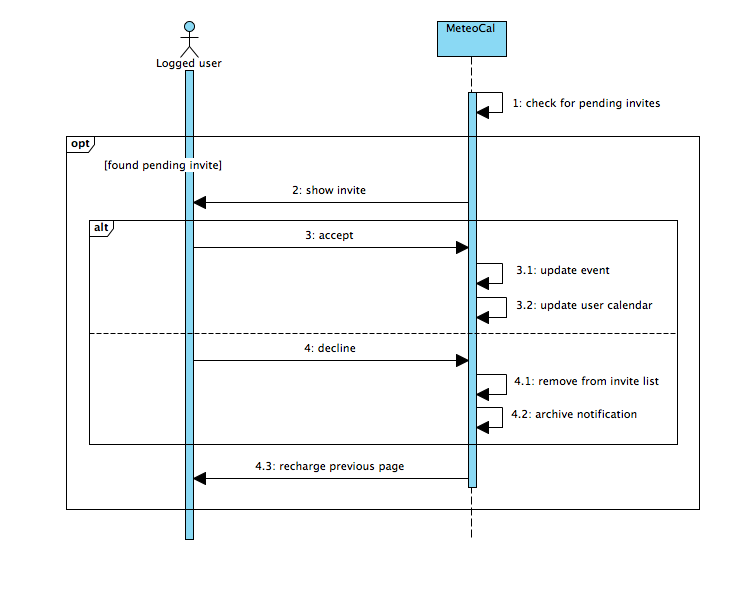
\includegraphics[width=\linewidth]{./Sequence_diag/USC009.png}
\caption[USC009]{USC009 - Decline an event invite}
\label{fig:USC009}
\end{figure}

\clearpage
\subsubsection{Search the calendar of another user}

\begin{tabular}[h]{| p{3cm} | p{10cm} |}
\hline \multicolumn{2}{|c|}{\textbf{Search the calendar of another user}} \\ 
\hline Code & USC010\\ 
\hline Description & A user searches the page of another user to see his calendar \\
\hline Goal & G4: Allow users to see other users public calendar\\
\hline Assumptions  & \begin{enumerate}
\item both users are registered
\item the user who performs the search is logged in
\item the user who performs the search knows the name/username of the other
\end{enumerate} \\
\hline Actors &  \begin{enumerate}
\item Logged user
\end{enumerate} \\
\hline Entry condition & The user is on a MeteoCal page\\
\hline Exit condition & The user finds the desired calendar\\
\hline Flow of events & \begin{enumerate}
\item The user clicks on the search bar and writes the other user name (or user name)
\item He presses enter
\item The systems shows a result page with all the people with the selected name
\item The user scrolls the bar and search the other one looking at the displayed details (name, username, mail)
\item The user finds the desired user and press the related “see calendar” button
\end{enumerate}\\
\hline Exceptions & No users found during the search \\
\hline Special requirements & \\
\hline Nonfunctional requirements & \\
\hline
\end{tabular}
\begin{figure}[h]
\centering
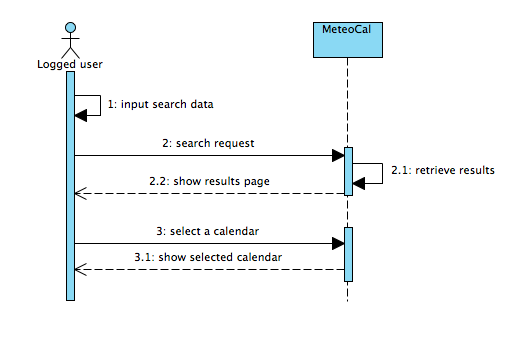
\includegraphics[width=\linewidth]{./Sequence_diag/USC010.png}
\caption[USC010]{USC010 - Search the calendar of another user}
\label{fig:USC010}
\end{figure}

\clearpage
\subsubsection{Browse another user calendar} 

\begin{tabular}[h]{| p{3cm} | p{10cm} |} 
\hline \multicolumn{2}{|c|}{\textbf{Browse another user calendar}} \\  
\hline Code & USC011\\  
\hline Description & Describing how a user navigate through another user's calendar\\ 
\hline Goal & \begin{itemize}
\item G4: Allow users to see other users public calendar
\item G5: Allow users to see other users public events details
\end{itemize}\\ 
\hline Assumptions  & \begin{enumerate} 
\item both users are registered
\item the second user has a public calendar with at least a public event
\item the first user has performed a search 
\end{enumerate} \\ 
\hline Actors &  \begin{enumerate} 
\item Logged user
\end{enumerate} \\ 
\hline Entry condition & The user has clicked on the “see calendar” button of a search result\\ 
\hline Exit condition & The user who performs the search finds the information he needs\\ 
\hline Flow of events & \begin{enumerate} 
\item The user goes through the selected user calendar
\item The user accesses the event details of a public event by clicking on the event box in the calendar
\item The systems retrieves the information about the event and shows them to the user in a box on the right of the calendar
\end{enumerate}\\ 
\hline Exceptions & \begin{itemize}
\item The user clicks on a private event
\item The “searched” user has a private calendar
\end{itemize}\\ 
\hline Special requirements & \\ 
\hline Nonfunctional requirements & \\
\hline 
\end{tabular} 
\begin{figure}[h]
\centering
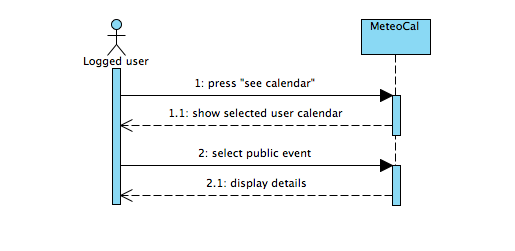
\includegraphics[width=\linewidth]{./Sequence_diag/USC011.png}
\caption[USC011]{USC011 - Browse another user calendar}
\label{fig:USC011}
\end{figure}

\clearpage
\subsubsection{Receive bad weather alert} 

\begin{tabular}[h]{| p{3cm} | p{10cm} |} 
\hline \multicolumn{2}{|c|}{\textbf{Receive bad weather alert}} \\  
\hline Code & USC012\\  
\hline Description & The user receives a bad weather alert with one day of advance from the event\\ 
\hline Goal & G6: Send a notification to all the participants one day in advance in case a bad weather\\ 
\hline Assumptions  & \begin{enumerate} 
\item the user is registered
\item the user is going to take part in an outdoor event on the following day 
\item the weather forecasts for the following day are bad
\item the user has not answered to the notification yet
\end{enumerate} \\ 
\hline Actors &  \begin{enumerate} 
\item Logged user
\end{enumerate} \\ 
\hline Entry condition & The user is on a MeteoCal page and he receives a notification\\ 
\hline Exit condition & The notification disappears\\ 
\hline Flow of events & \begin{enumerate} 
\item The user logins into MeteoCal
\item The system checks the user's outdoor events: if an event of the following day has bad weather he sends a notification to the user
\item The user receives the notification (which is shown “over” the MeteoCal page he's currently on)
\item The user presses the “got it” button
\item The notification disappears
\end{enumerate}\\ 
\hline Exceptions & \begin{itemize}
\item The user exits MeteoCal before after receiving the notification but before clicking on the “got it “ button
\item The user exits MeteoCal before he receives the notification
\end{itemize}\\ 
\hline Special requirements & \\ 
\hline Nonfunctional requirements & \\
\hline 
\end{tabular} 
\begin{figure}[h]
\centering
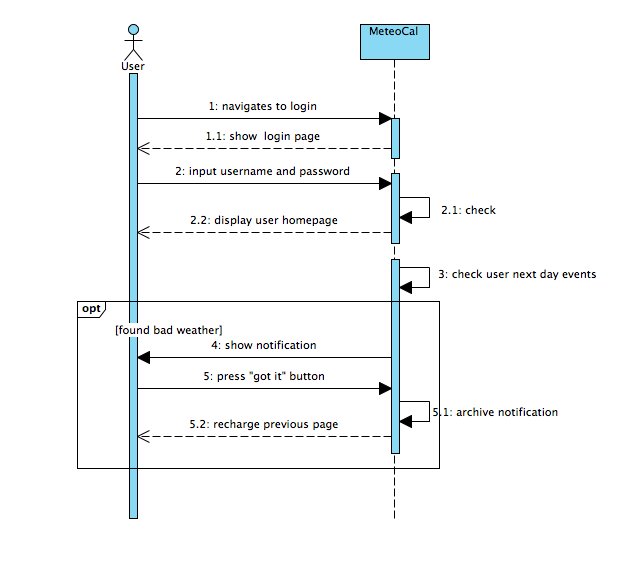
\includegraphics[width=\linewidth]{./Sequence_diag/USC012.png}
\caption[USC012]{USC012 - Receive bad weather alert}
\label{fig:USC012}
\end{figure}

\clearpage
\subsubsection{Propose a sunny day} 

\begin{longtable}[h]{| p{3cm} | p{10cm} |} 
\hline \multicolumn{2}{|c|}{\textbf{Propose a sunny day}} \\  
\hline Code & USC013 \\  
\hline Description & If three days before the event its weather forecasts are bad, the system warns the creator and suggests him to change the date to the closest sunny day. The user can move the event or leave it on the scheduled day\\ 
\hline Goal & G7: Propose an alternative schedule to the event creator three day in advance in case of bad weather\\ 
\hline Assumptions  & \begin{enumerate} 
\item the user is registered 
\item the user created an event
\item there are bad weather forecasts for the event
\item the event will take place after three days
\item the user accesses MeteoCal for the first time in that day
\end{enumerate} \\ 
\hline Actors &  \begin{enumerate} 
\item registered user 
\end{enumerate} \\ 
\hline Entry condition & The user accesses MeteoCal\\ 
\hline Exit condition & The systems has updated the event information or archived the notification\\ 
\hline Flow of events & \begin{enumerate} 
\item The user accesses MeteoCall
\item The systems checks the forecasts for the user outdoor events that will take place after three days
\item If it finds one event with bad weather forecasts it looks for the closest sunny day
\item Once found the sunny day the system sends the notification
\item The user, who's still on a MeteoCal page, receives the notification (shown over his current page)
\item The user selects whether to postpone the event or ignore the notification (“move” button, “ignore” button)
\item If necessary the systems updates the event details and generates the notifications for the participants
\end{enumerate}\\ 
\hline Exceptions & \begin{itemize}
\item The user exits MeteoCal after receiving the notification but before clicking on the “got it“ button.
\item The user exits MeteoCal before he receives the notification.
\item The system is not able to find any close sunny day.
\item The closest sunny event is full of other events.
\end{itemize}\\ 
\hline Special requirements &\\ 
\hline Nonfunctional requirements &\\
\hline 
\end{longtable} 
\begin{figure}[h]
\centering
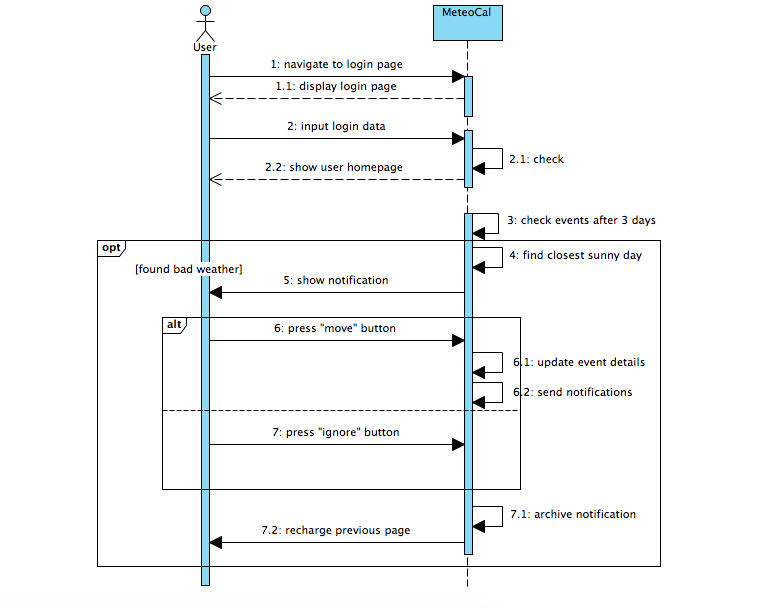
\includegraphics[width=\linewidth]{./Sequence_diag/USC013.png}
\caption[USC013]{USC013 - Propose a sunny day}
\label{fig:USC013}
\end{figure}

\clearpage
\subsubsection{Receive date changed notification} 

\begin{tabular}[h]{| p{3cm} | p{10cm} |} 
\hline \multicolumn{2}{|c|}{\textbf{Receive date changed notification}} \\  
\hline Code & USC014\\  
\hline Description & When the creator of an event changes its scheduled date due to bad weather all the participants are notified\\ 
\hline Goal & G9: Notify all the event's participant in case the creator changes some details\\ 
\hline Assumptions  & \begin{enumerate} 
\item the user is registered 
\item he accepted the invite to an event 
\item the creator changed the date of the event for bad weather conditions 
\item the user accesses MeteoCal for the  first time after the creator moved the event
\end{enumerate} \\ 
\hline Actors &  \begin{enumerate} 
\item registered user 
\end{enumerate} \\ 
\hline Entry condition & The user receives a notification\\ 
\hline Exit condition & The systems archives the notification\\ 
\hline Flow of events & \begin{enumerate} 
\item The user logins and enters in MeteoCal for the first time after the event creator moved its date
\item The system checks if there are “date-changed” notification pending for the user
\item The systems shows the notification
\item The user clicks on the “got it” button
\item The system deletes the notification
\end{enumerate}\\ 
\hline Exceptions & \begin{itemize}
\item The user exits MeteoCal before after receiving the notification but before clicking on the “got it“ button
\item The user exits MeteoCal before he receives the notification
\end{itemize}\\ 
\hline Special requirements & \\ 
\hline Nonfunctional requirements & \\
\hline 
\end{tabular} 
\begin{figure}[h]
\centering
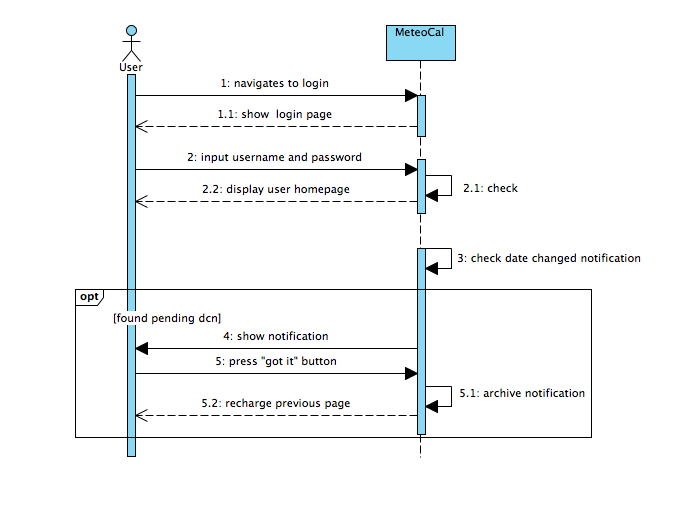
\includegraphics[width=\linewidth]{./Sequence_diag/USC014.png}
\caption[USC014]{USC014 - Receive date changed notification}
\label{fig:USC014}
\end{figure}

\clearpage
\subsubsection{Change data} 

\begin{tabular}[h]{| p{3cm} | p{10cm} |} 
\hline \multicolumn{2}{|c|}{\textbf{Change data}} \\  
\hline Code & USC015 \\  
\hline Description & A user accesses his settings page and change his password and his email address\\ 
\hline Goal & G10: Allow users to modify their data\\ 
\hline Assumptions  & \begin{enumerate} 
\item the user is logged
\end{enumerate} \\ 
\hline Actors &  \begin{enumerate} 
\item Logged user
\end{enumerate} \\ 
\hline Entry condition & The user decides to change his personal details\\ 
\hline Exit condition & The system has successfully updated the user information\\ 
\hline Flow of events & \begin{enumerate} 
\item The user press “settings button”
\item The system shows him the personal information page
\item The user types in the relative box the new mail
\item The user types in the relative box the old password and the new one
\item The user presses the “save” button
\item The system checks the old password
\item The system saves the updated information
\item The system shows to personal information page with the new details 
\end{enumerate}\\ 
\hline Exceptions & \begin{itemize}
\item The user does not type a valid email address.
\item The user uses the wrong boxes.
\item The user writes the old password.
\item The user exits before saving
\end{itemize}\\ 
\hline Special requirements &\\ 
\hline Nonfunctional requirements &\\ 
\hline 
\end{tabular} 
\begin{figure}[h]
\centering
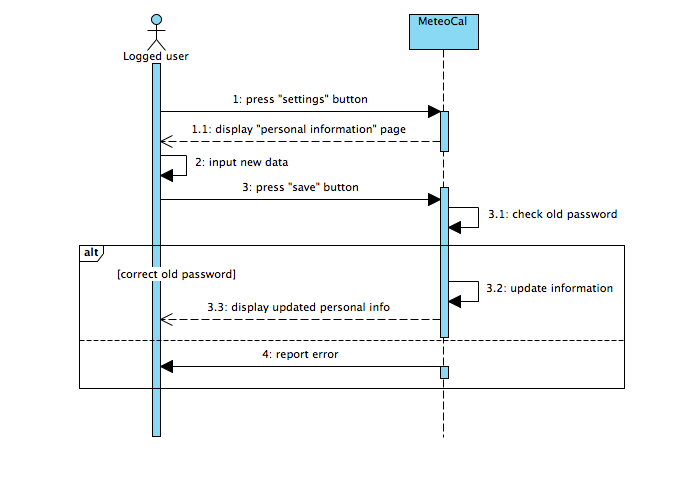
\includegraphics[width=\linewidth]{./Sequence_diag/USC015.png}
\caption[USC015]{USC015 - Change data}
\label{fig:USC015}
\end{figure}

\clearpage
\subsubsection{Update weather forecasts} 

\begin{tabular}[h]{| p{3cm} | p{10cm} |} 
\hline \multicolumn{2}{|c|}{\textbf{Use case name}} \\  
\hline Code & USC016\\  
\hline Description & MeteoCal asks an external meteo service for updated weather forecasts for all the scheduled events\\ 
\hline Goal & \begin{itemize}
\item G7: Send a notification to all the participants one day in advance in case of bad weather
\item G8: Propose an alternative schedule to the event creator three day in advance in case of bad weather
\end{itemize}\\
\hline Assumptions  & \begin{enumerate} 
\item the systems has some user events in his database
\item the system has an interface to “speak” with an external weather forecasts service
\end{enumerate} \\ 
\hline Actors &  \begin{enumerate} 
\item external meteo service
\end{enumerate} \\ 
\hline Entry condition & The system has to update some forecasts\\ 
\hline Exit condition & The system saved the updated forecasts that are now available to users\\ 
\hline Flow of events & \begin{enumerate} 
\item The MeteoCal system generates a forecast request for the event that has to be updated
\item The forecast service answers providing new forecasts
\item The system update its record with the new data
\item The procedure is repeated for all the event that has to be updated
\end{enumerate}\\ 
\hline Exceptions & \begin{itemize}
\item  The external meteo service is not available
\item The external meteo service can’t provide new forecasts
\item The external meteo service can’t provide forecasts for the relevant place
\end{itemize}\\ 
\hline Special requirements &\\ 
\hline Nonfunctional requirements &\\ 
\hline 
\end{tabular} 
\begin{figure}[h]
\centering
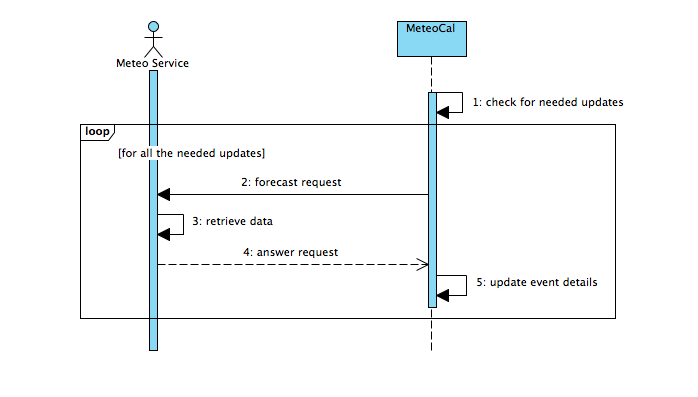
\includegraphics[width=\linewidth]{./Sequence_diag/USC016.png}
\caption[USC016]{USC016 - Update weather forecast}
\label{fig:USC016}
\end{figure}

\section{Performance requirements}
The software product requires that every web page shall download in 15 seconds or less.

\section{Design constraints}
The software product must be designed and implemented with JEE technologies, in particular
EJBs for the business logic.

\section{Software system attributes}

\subsection{Reliability}
The software product does not any reliability factors because in case of malfunction it will
cause minor inconveniences.

\subsection{Availability}
The system shall be available 24 hours per day, 365 days per year.

\subsection{Security}
The software product must provide secure storage of the passwords of its users. This can be
achieved by using any cryptographic techniques.

\subsection{Maintainability}
The database must be backed up periodically, so that new connection and skill data is not lost
in case of malfunction.

\subsection{Portability}
The software product can be installed in any operating system that supports the JVM and its dependent components.

\section{Other requirements}
The software product must provide understandable messages in text form in the event of
errors, and instruct the user on what to do.

\clearpage
\part{Appendixes}

\clearpage
\tableofcontents
\end{document}
\sub